\chapter{Steuerwerk}
\label{chap:Steuerwerk}

\section{Allgemeine Funktion}

Das Steuerwerk ist das zentrale Element der CPU, das für die Koordination aller Komponenten verantwortlich ist.
Es erzeugt die Steuersignale, um Datenflüsse und Operationen innerhalb der Architektur zu steuern.
Außerdem kontrolliert es den Programmzähler (PC) und verwaltet die Adressierung von Befehlen und Daten im RAM.
\\\\
Das Steuerwerk erhält Statussignale (z. B. Carry, Overflow, Zero), die von der ALU generiert werden, und
passt die Steuerung an, um Instruktionen korrekt auszuführen.
\\\\
Im Folgenden werden die Ein- und Ausgänge des Steuerwerks detailliert beschrieben.

\section{Eingänge}
\begin{table}[H]
    \centering
    \begin{tabular}{|l|p{10cm}|}
        \hline
        \textbf{Signal}   & \textbf{Beschreibung}                                                           \\ \hline
        \textbf{Reset}    & Setzt das Steuerwerk in den Anfangszustand zurück.                              \\ \hline
        \textbf{BLA}      & Busy-Look-Ahead-Signal zur Vorhersage von Busy-Zuständen in der ALU.            \\ \hline
        \textbf{Busy}     & Statussignal der ALU, das die ALU momentan mit einer Operation beschäftigt ist. \\ \hline
        \textbf{Carry}    & Flag, das von der ALU bei einem Übertrag (Carry) gesetzt wird.                  \\ \hline
        \textbf{Overflow} & Flag, das bei einem Überlauf (Overflow) während ALU-Operationen gesetzt wird.   \\ \hline
        \textbf{Zero}     & Flag, das gesetzt wird, wenn das ALU-Ergebnis null ist.                         \\ \hline
        \textbf{C3..0}    & Die von der ALU auszuführende Operation.                                        \\ \hline
    \end{tabular}
    \caption{Eingänge des Steuerwerks}
\end{table}

\noindent Die Flags werden in \autoref{TODO} ausführlich erklärt.
\\\\
Die genannten Eingänge sind nötig für die Entscheidung, welche Operation als nächstes durchgeführt wird. \\
Das Steuerwerk nutzt diese Signale, um Befehle effektiv zu koordinieren und auszuführen und generiert die im folgenden Abschnitt aufgeführten Ausgaben.

\section{Ausgänge}
\begin{table}[H]
    \centering
    \begin{tabular}{|l|p{10cm}|}
        \hline
        \textbf{Signal}      & \textbf{Beschreibung}                                                                                           \\ \hline
        \textbf{WriteA}      & Schreibt Operanden aus dem RAM in Register A.                                                                   \\ \hline
        \textbf{WriteRAM}    & Schreibt das Ergebnis von Register A in den RAM.                                                                \\ \hline
        \textbf{WriteADR1}   & Speichert die 4 MSB-Adressbits (ADR7..4) aus dem RAM im Adressregister (RegADR).                                \\ \hline
        \textbf{WriteADR2}   & Speichert die 4 LSB-Adressbits (ADR3..0) aus dem RAM im Adressregister (RegADR).                                \\ \hline
        \textbf{WriteOP}     & Schreibt die aktuelle Operation in das OpReg während des Fetch-Zyklus.                                          \\ \hline
        \textbf{!PC\_LD}     & Lädt den Programmzähler (PC).                                                                                   \\ \hline
        \textbf{!PC\_EN}     & Aktiviert den Programmzähler, damit er hoch- oder runterzählen kann.                                            \\ \hline
        \textbf{PC\_UP}      & Gibt an, ob der PC hochzählt (\texttt{PC\_UP=1}) oder runterzählt (\texttt{PC\_UP=0}).                          \\ \hline
        \textbf{RegADRtoRAM} & Bestimmt, ob die Adresse im RAM von RegADR oder dem Programmzähler kommt. Bei \texttt{RegADRtoRAM = 1}
        Wird die Adresse vom RegADR übertragen.                                                                                                \\ \hline
        \textbf{ALUStart}    & Startet die ALU zur Ausführung einer Operation.                                                                 \\ \hline
        \textbf{SWR}         & Tauscht den Inhalt von Register A und Register B, die beim Starten der ALU die Operanden in die ALU übertragen. \\ \hline
    \end{tabular}
    \caption{Ausgänge des Steuerwerks}
\end{table}

Diese Ausgänge beeinflussen die ganze CPU und ermöglichen die Steuerung der internen Prozesse.
Die Interaktion zwischen den Ein- und Ausgangssignalen gewährleistet dabei die korrekte Ausführung aller Operationen.


\section{Automat}
Der Zustand des Steuerwerks wird mithilfe eines Moore-Automaten gesteuert, der auf den Eingabesignalen und internen Zuständen basiert.

\textbf{Wichtig zu beachten:}
\begin{itemize}
    \item Nicht explizit beschriebene Zustandsausgaben sind 0.
    \item X bedeutet don’t care: Das Signal kann auf 1 oder 0 anliegen.
    \item Ein Wert von 1 auf den Pfeilen signalisiert, dass die Transition ohne zusätzliche Bedingungen erfolgen kann.
\end{itemize}

\begin{figure}[H]
    \centering
    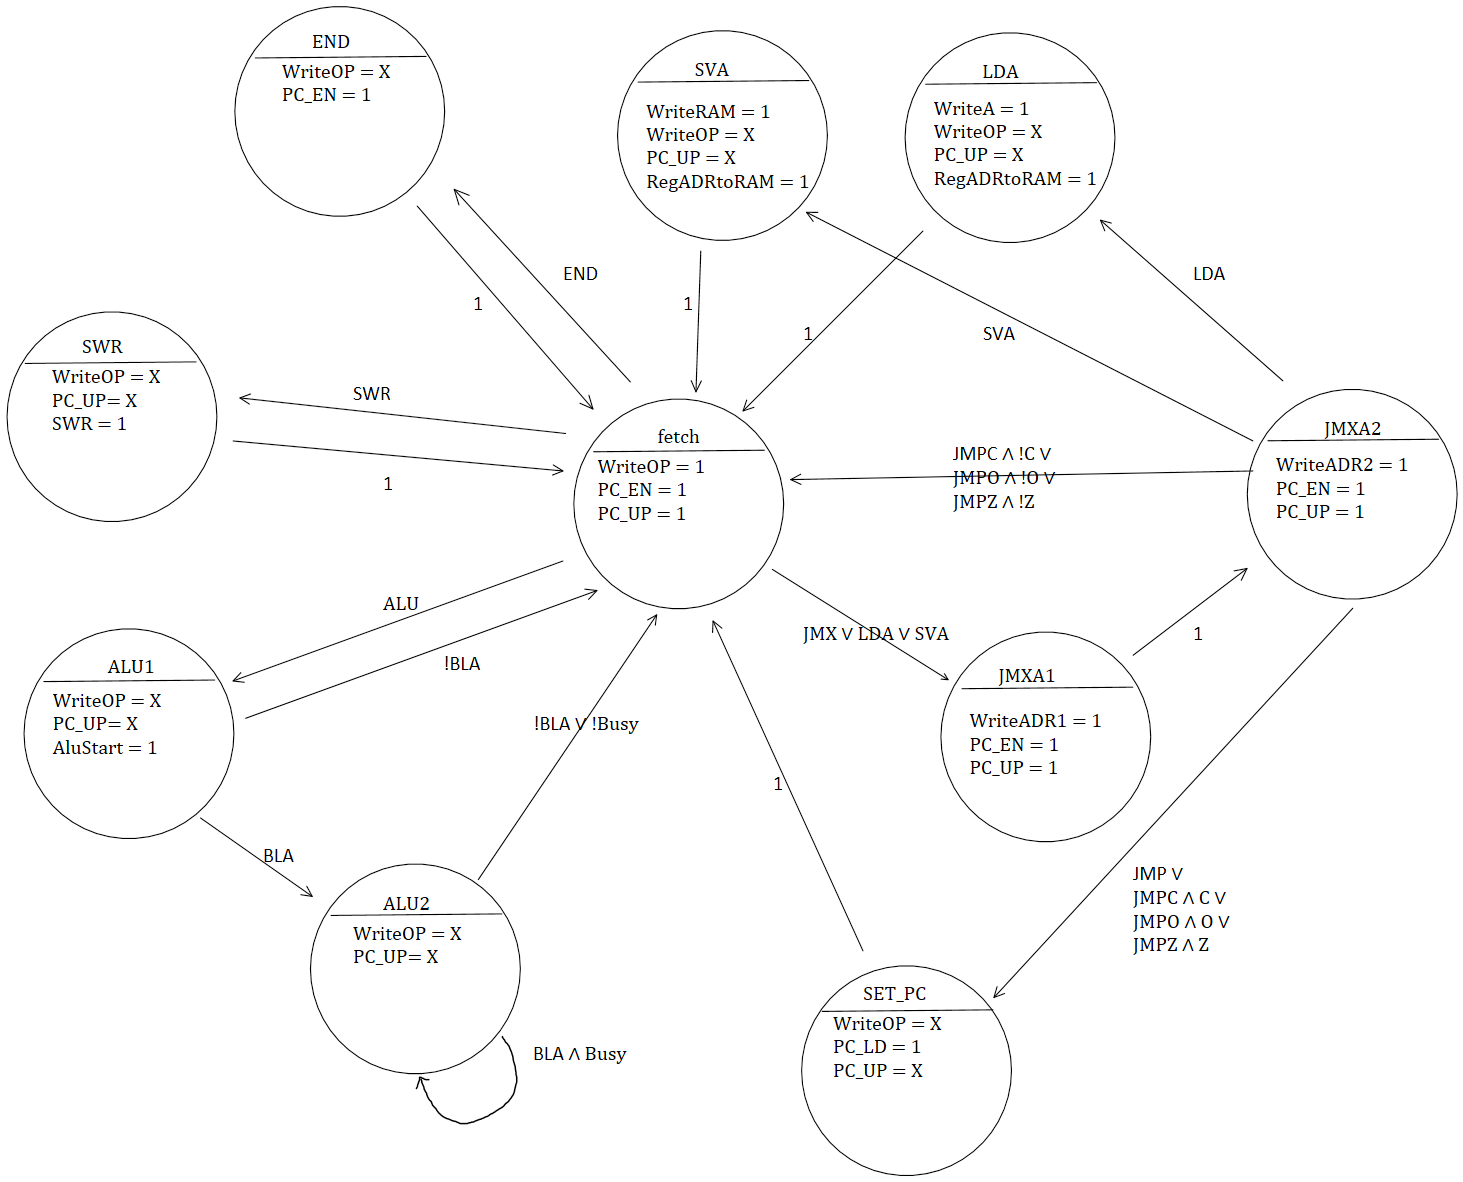
\includegraphics[scale=0.279]
    {content/figures/SW_Zustaende}
    \caption{Zustandsautomat Steuerwerk}
    \label{fig:SW_Zustaende}
\end{figure}


\section{Zustandscodierung}
\label{sec:Zustandscodierung}

\begin{table} [H]
    \centering
    \begin{tabular}{|l|c|c|c|c|}
        \hline
        \multirow{2}{*}{\textbf{Zustand}} & \multicolumn{4}{c}{\textbf{Codierung}}                \\

                                          & Q3                                     & Q2 & Q1 & Q0 \\
        \hline
        \textbf{Fetch}                    & 0                                      & 0  & 0  & 0  \\
        \hline
        \textbf{SET\_PC}                  & 0                                      & 0  & 1  & 0  \\
        \hline
        \textbf{ALU1}                     & 0                                      & 1  & 0  & 0  \\
        \hline
        \textbf{ALU2}                     & 0                                      & 1  & 0  & 1  \\
        \hline
        \textbf{JMXA1}                    & 1                                      & 0  & 0  & 0  \\
        \hline
        \textbf{JMXA2}                    & 1                                      & 0  & 0  & 1  \\
        \hline
        \textbf{LDA}                      & 1                                      & 1  & 0  & 0  \\
        \hline
        \textbf{SVA}                      & 1                                      & 1  & 0  & 1  \\
        \hline
        \textbf{SWR}                      & 1                                      & 1  & 1  & 0  \\
        \hline
        \textbf{END}                      & 1                                      & 1  & 1  & 1  \\
        \hline
        \textbf{Don´t Care}               & -                                      & -  & -  & -  \\
        \hline
    \end{tabular}
    \caption{Zustandscodierung des Steuerwerks}
    \label{tab:Zustandscodierung}
\end{table}

\noindent \textbf{Wichtig} Alle nicht definierten Zustände sind "Don´t Care"


\section{Operationen und Anweisungen}
Das Steuerwerk kann Mithilfe der ALU folgende Funktionen ausführen:
\begin{itemize}
    \item \textbf{Logisch} AND, OR, NOT
    \item \textbf{Arithmetisch} Addition (ADD), Subtraktion (SUB), Multiplikation (MUL).
    \item \textbf{Sprung} JMP, JMPC (für Carry), JMPO (für Overflow), JMPZ (für Zero).
    \item \textbf{Speicher} LDA (Load Register A), SVA (Save Register A).
    \item \textbf{Spezial} SWR (Switch Registers), END.
\end{itemize}

\noindent Dabei wird jede Operation durch eine Kombination der Steuerbits \texttt{C3..0} definiert.

\begin{table}[H]
    \centering
    \begin{tabular}{|p{0.5cm}|p{0.5cm}|p{0.5cm}|p{0.5cm}|p{2.7cm}|p{6cm}|}
        \hline
        \multicolumn{4}{|c|}{\textbf{Codierung}} & \textbf{Operation} & \textbf{Beschreibung}                                                                                                                         \\

        C3                                       & C2                 & C1                    & C0 &          &                                                                                                       \\
        \hline
        0                                        & 0                  & 0                     & 0  & AND      & Bitweises UND (\boldmath{$A \land B$})                                                                \\
        \hline
        0                                        & 0                  & 0                     & 1  & OR       & Bitweises ODER (\boldmath{$A \lor B$})                                                                \\
        \hline
        0                                        & 0                  & 1                     & 0  & NOT      & Invertiert A (\boldmath{$\neg A$})                                                                    \\
        \hline
        0                                        & 0                  & 1                     & 1  & ADD      & Binäre Addition (\boldmath{$A + B$})                                                                  \\
        \hline

        \hline
        0                                        & 1                  & 0                     & 0  & SUB      & Binäre Subtraktion (\boldmath{$A - B$})                                                               \\
        \hline
        0                                        & 1                  & 0                     & 1  & MUL      & Binäre Multiplikation (\boldmath{$A \times B$})                                                       \\
        \hline
        0                                        & 1                  & 1                     & 0  & RESERVED & \textit{Frei im PROM der ALU programmierbar}                                                          \\
        \hline
        0                                        & 1                  & 1                     & 1  & RESERVED & \textit{Frei im PROM der ALU programmierbar}                                                          \\
        \hline
        \hline
        1                                        & 0                  & 0                     & 0  & JMP      & \textbf{TODO}                                                                                         \\
        \hline
        1                                        & 0                  & 0                     & 1  & JMPC     & \textbf{TODO}                                                                                         \\
        \hline
        1                                        & 0                  & 1                     & 0  & JMPO     & \textbf{TODO}                                                                                         \\
        \hline
        1                                        & 0                  & 1                     & 1  & JMPZ     & \textbf{TODO}                                                                                         \\
        \hline

        \hline
        1                                        & 1                  & 0                     & 0  & LDA      & Schreibt den 4-Bit Operanden vom RAM in Register A (\boldmath{$RAM3..0 \rightarrow A$})               \\
        \hline
        1                                        & 1                  & 0                     & 1  & SVA      & Schreibt das 4-Bit Ergebnis von Register A in den RAM (\boldmath{$A \rightarrow RAM3..0$})            \\
        \hline
        1                                        & 1                  & 1                     & 0  & SWR      & Tauscht den Inhalt von Register A und Register B (\boldmath{$A \rightarrow B \land B \rightarrow A$}) \\
        \hline
        1                                        & 1                  & 1                     & 1  & END      & \textbf{TODO}  Beenden der Rechnenoperation                                                           \\
        \hline
    \end{tabular}
    \caption{Unterstützte Operationen}
    \label{fig:Unterstützte Operationen}
\end{table}

\section{Gleichungen der Transitionen}
\texttt{D3..0} stellen Ausgänge der Transitionsfunktion dar und definieren die Bedingungen, unter denen
die Eingänge der Flip-Flops gesetzt werden, um den nächsten Zustand im Steuerwerk zu erreichen.
\begin{itemize}
    \item \textbf{D3} = $(\overline{R} \land \overline{Q2} \land \overline{Q1} \land \overline{Q0} \land C3) \lor (\overline{R} \land Q3 \land \overline{Q2} \land \overline{Q0}) \lor (\overline{R} \land Q3 \land \overline{Q2} \land C2).$

    \item \textbf{D2} = $(\overline{R} \land \overline{Q3} \land \overline{Q2} \land \overline{Q1} \land \overline{C3}) \lor (\overline{R} \land \overline{Q3} \land \overline{Q2} \land \overline{Q1} \land C2 \land C1) \lor \\
              (\overline{R} \land \overline{Q3} \land Q2 \land \overline{Q0} \land BLA) \lor (\overline{R} \land \overline{Q2} \land Q0 \land C2) \lor \\
              (\overline{R} \land \overline{Q3} \land Q2 \land BLA \land Busy). $

    \item \textbf{D1} = $(\overline{R} \land \overline{Q3} \land \overline{Q2} \land \overline{Q1} \land C3 \land C2 \land C1) \lor (\overline{R} \land \overline{Q2} \land Q0 \land \overline{C2} \land \overline{C1} \land \overline{C0}) \lor \\
              (\overline{R} \land \overline{Q2} \land Q0 \land \overline{C2} \land \overline{C1} \land Carry) \lor (\overline{R} \land \overline{Q2} \land Q0 \land C1 \land C0 \land Zero) \lor \\
              (\overline{R} \land \overline{Q2} \land Q0 \land \overline{C2} \land \overline{C0} \land Overflow). $

    \item \textbf{D0} = $(\overline{R} \land \overline{Q2} \land \overline{Q1} \land C3 \land C2 \land C1 \land C0) \lor (\overline{R} \land Q3 \land \overline{Q2} \land \overline{Q0} \land BLA) \lor \\
              (\overline{R} \land Q3 \land \overline{Q2} \land \overline{Q0}) \lor (\overline{R} \land \overline{Q3} \land Q2 \land BLA \land Busy) \lor \\
              (\overline{R} \land Q3 \land \overline{Q2} \land C2 \land C0)$.
\end{itemize}



\section{Gleichungen der Outputs}
Die Gleichungen für die Outputs des Steuerwerks legen fest, welche Signale aktiviert werden,
abhängig von den aktuellen Zuständen der Steuerbits \texttt{Q3..0}.
\begin{itemize}
    \item \textbf{WriteA}
          ($Q3 \land Q2 \land \overline Q1 \land \overline Q0$)

    \item \textbf{WriteRAM}
          ($Q3 \land Q2 \land \overline Q1 \land Q0$)

    \item \textbf{WriteADR1}
          ($Q3 \land \overline Q2 \land \overline Q0$)

    \item \textbf{WriteADR2}
          ($\overline Q2 \land Q0$)

    \item \textbf{WriteOP}
          $\overline Q3$

    \item \textbf{!PC-LD}
          $\overline Q1 \lor Q2$

    \item \textbf{!PC-EN}
          $(Q2 \land \overline Q1) \lor
              (Q1 \land \overline Q0)$

    \item \textbf{PC-UP}
          $!Q1$

    \item \textbf{RegADRtoRAM}
          ($Q3 \land Q2 \land \overline Q1$)

    \item \textbf{AluStart}
          ($\overline Q3 \land Q2 \land \overline Q0$)

    \item \textbf{SWR}
          ($Q2 \land Q1 \land \overline Q0$)
\end{itemize}




